\documentclass[]{article}
\usepackage{lmodern}
\usepackage{amssymb,amsmath}
\usepackage{ifxetex,ifluatex}
\usepackage{fixltx2e} % provides \textsubscript
\ifnum 0\ifxetex 1\fi\ifluatex 1\fi=0 % if pdftex
  \usepackage[T1]{fontenc}
  \usepackage[utf8]{inputenc}
\else % if luatex or xelatex
  \ifxetex
    \usepackage{mathspec}
  \else
    \usepackage{fontspec}
  \fi
  \defaultfontfeatures{Ligatures=TeX,Scale=MatchLowercase}
\fi
% use upquote if available, for straight quotes in verbatim environments
\IfFileExists{upquote.sty}{\usepackage{upquote}}{}
% use microtype if available
\IfFileExists{microtype.sty}{%
\usepackage{microtype}
\UseMicrotypeSet[protrusion]{basicmath} % disable protrusion for tt fonts
}{}
\usepackage[margin=1in]{geometry}
\usepackage{hyperref}
\hypersetup{unicode=true,
            pdftitle={Curs Biostatistica 2017 - Laborator 5 \& 6},
            pdfborder={0 0 0},
            breaklinks=true}
\urlstyle{same}  % don't use monospace font for urls
\usepackage{color}
\usepackage{fancyvrb}
\newcommand{\VerbBar}{|}
\newcommand{\VERB}{\Verb[commandchars=\\\{\}]}
\DefineVerbatimEnvironment{Highlighting}{Verbatim}{commandchars=\\\{\}}
% Add ',fontsize=\small' for more characters per line
\usepackage{framed}
\definecolor{shadecolor}{RGB}{248,248,248}
\newenvironment{Shaded}{\begin{snugshade}}{\end{snugshade}}
\newcommand{\KeywordTok}[1]{\textcolor[rgb]{0.13,0.29,0.53}{\textbf{{#1}}}}
\newcommand{\DataTypeTok}[1]{\textcolor[rgb]{0.13,0.29,0.53}{{#1}}}
\newcommand{\DecValTok}[1]{\textcolor[rgb]{0.00,0.00,0.81}{{#1}}}
\newcommand{\BaseNTok}[1]{\textcolor[rgb]{0.00,0.00,0.81}{{#1}}}
\newcommand{\FloatTok}[1]{\textcolor[rgb]{0.00,0.00,0.81}{{#1}}}
\newcommand{\ConstantTok}[1]{\textcolor[rgb]{0.00,0.00,0.00}{{#1}}}
\newcommand{\CharTok}[1]{\textcolor[rgb]{0.31,0.60,0.02}{{#1}}}
\newcommand{\SpecialCharTok}[1]{\textcolor[rgb]{0.00,0.00,0.00}{{#1}}}
\newcommand{\StringTok}[1]{\textcolor[rgb]{0.31,0.60,0.02}{{#1}}}
\newcommand{\VerbatimStringTok}[1]{\textcolor[rgb]{0.31,0.60,0.02}{{#1}}}
\newcommand{\SpecialStringTok}[1]{\textcolor[rgb]{0.31,0.60,0.02}{{#1}}}
\newcommand{\ImportTok}[1]{{#1}}
\newcommand{\CommentTok}[1]{\textcolor[rgb]{0.56,0.35,0.01}{\textit{{#1}}}}
\newcommand{\DocumentationTok}[1]{\textcolor[rgb]{0.56,0.35,0.01}{\textbf{\textit{{#1}}}}}
\newcommand{\AnnotationTok}[1]{\textcolor[rgb]{0.56,0.35,0.01}{\textbf{\textit{{#1}}}}}
\newcommand{\CommentVarTok}[1]{\textcolor[rgb]{0.56,0.35,0.01}{\textbf{\textit{{#1}}}}}
\newcommand{\OtherTok}[1]{\textcolor[rgb]{0.56,0.35,0.01}{{#1}}}
\newcommand{\FunctionTok}[1]{\textcolor[rgb]{0.00,0.00,0.00}{{#1}}}
\newcommand{\VariableTok}[1]{\textcolor[rgb]{0.00,0.00,0.00}{{#1}}}
\newcommand{\ControlFlowTok}[1]{\textcolor[rgb]{0.13,0.29,0.53}{\textbf{{#1}}}}
\newcommand{\OperatorTok}[1]{\textcolor[rgb]{0.81,0.36,0.00}{\textbf{{#1}}}}
\newcommand{\BuiltInTok}[1]{{#1}}
\newcommand{\ExtensionTok}[1]{{#1}}
\newcommand{\PreprocessorTok}[1]{\textcolor[rgb]{0.56,0.35,0.01}{\textit{{#1}}}}
\newcommand{\AttributeTok}[1]{\textcolor[rgb]{0.77,0.63,0.00}{{#1}}}
\newcommand{\RegionMarkerTok}[1]{{#1}}
\newcommand{\InformationTok}[1]{\textcolor[rgb]{0.56,0.35,0.01}{\textbf{\textit{{#1}}}}}
\newcommand{\WarningTok}[1]{\textcolor[rgb]{0.56,0.35,0.01}{\textbf{\textit{{#1}}}}}
\newcommand{\AlertTok}[1]{\textcolor[rgb]{0.94,0.16,0.16}{{#1}}}
\newcommand{\ErrorTok}[1]{\textcolor[rgb]{0.64,0.00,0.00}{\textbf{{#1}}}}
\newcommand{\NormalTok}[1]{{#1}}
\usepackage{longtable,booktabs}
\usepackage{graphicx,grffile}
\makeatletter
\def\maxwidth{\ifdim\Gin@nat@width>\linewidth\linewidth\else\Gin@nat@width\fi}
\def\maxheight{\ifdim\Gin@nat@height>\textheight\textheight\else\Gin@nat@height\fi}
\makeatother
% Scale images if necessary, so that they will not overflow the page
% margins by default, and it is still possible to overwrite the defaults
% using explicit options in \includegraphics[width, height, ...]{}
\setkeys{Gin}{width=\maxwidth,height=\maxheight,keepaspectratio}
\IfFileExists{parskip.sty}{%
\usepackage{parskip}
}{% else
\setlength{\parindent}{0pt}
\setlength{\parskip}{6pt plus 2pt minus 1pt}
}
\setlength{\emergencystretch}{3em}  % prevent overfull lines
\providecommand{\tightlist}{%
  \setlength{\itemsep}{0pt}\setlength{\parskip}{0pt}}
\setcounter{secnumdepth}{5}
% Redefines (sub)paragraphs to behave more like sections
\ifx\paragraph\undefined\else
\let\oldparagraph\paragraph
\renewcommand{\paragraph}[1]{\oldparagraph{#1}\mbox{}}
\fi
\ifx\subparagraph\undefined\else
\let\oldsubparagraph\subparagraph
\renewcommand{\subparagraph}[1]{\oldsubparagraph{#1}\mbox{}}
\fi

%%% Use protect on footnotes to avoid problems with footnotes in titles
\let\rmarkdownfootnote\footnote%
\def\footnote{\protect\rmarkdownfootnote}

%%% Change title format to be more compact
\usepackage{titling}

% Create subtitle command for use in maketitle
\newcommand{\subtitle}[1]{
  \posttitle{
    \begin{center}\large#1\end{center}
    }
}

\setlength{\droptitle}{-2em}
  \title{Curs Biostatistica 2017 - Laborator 5 \& 6}
  \pretitle{\vspace{\droptitle}\centering\huge}
  \posttitle{\par}
\subtitle{Analiza de varianta - ANOVA}
  \author{}
  \preauthor{}\postauthor{}
  \date{}
  \predate{}\postdate{}

\usepackage{booktabs}
\usepackage{longtable}
\usepackage{framed,color}
\definecolor{shadecolor}{RGB}{248,248,248}

\ifxetex
  \usepackage{letltxmacro}
  \setlength{\XeTeXLinkMargin}{1pt}
  \LetLtxMacro\SavedIncludeGraphics\includegraphics
  \def\includegraphics#1#{% #1 catches optional stuff (star/opt. arg.)
    \IncludeGraphicsAux{#1}%
  }%
  \newcommand*{\IncludeGraphicsAux}[2]{%
    \XeTeXLinkBox{%
      \SavedIncludeGraphics#1{#2}%
    }%
  }%
\fi

\newenvironment{rmdblock}[1]
  {\begin{shaded*}
  \begin{itemize}
  \renewcommand{\labelitemi}{
    \raisebox{-.7\height}[0pt][0pt]{
      {\setkeys{Gin}{width=2em,keepaspectratio}\includegraphics{images/icons/#1}}
    }
  }
  \item
  }
  {
  \end{itemize}
  \end{shaded*}
  }
\newenvironment{rmdcaution}
  {\begin{rmdblock}{caution}}
  {\end{rmdblock}}
\newenvironment{rmdinsight}
  {\begin{rmdblock}{insight}}
  {\end{rmdblock}}
\newenvironment{rmdexercise}
  {\begin{rmdblock}{exercise}}
  {\end{rmdblock}}
\newenvironment{rmdtip}
  {\begin{rmdblock}{tip}}
  {\end{rmdblock}}

\begin{document}
\maketitle

{
\setcounter{tocdepth}{2}
\tableofcontents
}
\section{Analiză de varianță cu un factor (one-way
ANOVA)}\label{analiza-de-varianta-cu-un-factor-one-way-anova}

\begin{center}\rule{0.5\linewidth}{\linethickness}\end{center}

\begin{center}\rule{0.5\linewidth}{\linethickness}\end{center}

\subsection{Exemplul 1}\label{exemplul-1}

\begin{center}\rule{0.5\linewidth}{\linethickness}\end{center}

\begin{quote}
Vom analiza setul de date \texttt{Cushings} din pachetul \texttt{MASS}.
Sindromul \emph{Cushing} reprezintă o serie de semne și simptome ca
urmare a expunerii organismului pentru o perioadă îndelungată de timp la
o concentrație ridicată de cortizon (mai multe detalii
\href{http://www.csid.ro/boli-afectiuni/endocrinologie/sindromul-cushing-12821884/}{aici}
și \href{https://en.wikipedia.org/wiki/Cushing\%27s_syndrome}{aici}).
Pentru fiecare individ din eșantion, ratele de excreție urinară a doi
metaboliți steroizi sunt înregistrate: \emph{Tetrahydrocortisone} și
\emph{Pregnanetriol}. Variabila \emph{Type} arată tipul de sindrom
Cushing, acesta putând lua una din următoarele patru categorii:
\emph{adenom}
(\href{http://www.sfatulmedicului.ro/dictionar-medical/adenom_119}{a}),
\emph{hiperplazia bilaterală}
(\href{http://www.sfatulmedicului.ro/Afectiunile-suprarenalelor/hiperplazia-congenitala-a-glandelor-suprarenale_8123}{b}),
\emph{carcinom}
(\href{http://www.sfatulmedicului.ro/Cancer/ce-este-carcinomul_15473}{c})
și \emph{necunoscut} (u). Obiectivul este să investigăm dacă cele patru
tipuri de sindrom sunt diferite în raport cu excreția urinară de
\emph{Tetrahydrocortisone}.
\end{quote}

Începem prin a atașa setul de date \texttt{Cushings}:

\begin{Shaded}
\begin{Highlighting}[]
\KeywordTok{library}\NormalTok{(MASS)}
\KeywordTok{data}\NormalTok{(}\StringTok{"Cushings"}\NormalTok{)}
\KeywordTok{attach}\NormalTok{(Cushings)}
\end{Highlighting}
\end{Shaded}

\begin{longtable}[]{@{}ccc@{}}
\toprule
Tetrahydrocortisone & Pregnanetriol & Type\tabularnewline
\midrule
\endhead
3.1 & 11.70 & a\tabularnewline
3.0 & 1.30 & a\tabularnewline
1.9 & 0.10 & a\tabularnewline
3.8 & 0.04 & a\tabularnewline
4.1 & 1.10 & a\tabularnewline
1.9 & 0.40 & a\tabularnewline
8.3 & 1.00 & b\tabularnewline
3.8 & 0.20 & b\tabularnewline
3.9 & 0.60 & b\tabularnewline
7.8 & 1.20 & b\tabularnewline
9.1 & 0.60 & b\tabularnewline
15.4 & 3.60 & b\tabularnewline
7.7 & 1.60 & b\tabularnewline
6.5 & 0.40 & b\tabularnewline
5.7 & 0.40 & b\tabularnewline
13.6 & 1.60 & b\tabularnewline
10.2 & 6.40 & c\tabularnewline
9.2 & 7.90 & c\tabularnewline
9.6 & 3.10 & c\tabularnewline
53.8 & 2.50 & c\tabularnewline
15.8 & 7.60 & c\tabularnewline
5.1 & 0.40 & u\tabularnewline
12.9 & 5.00 & u\tabularnewline
13.0 & 0.80 & u\tabularnewline
2.6 & 0.10 & u\tabularnewline
30.0 & 0.10 & u\tabularnewline
20.5 & 0.80 & u\tabularnewline
\bottomrule
\end{longtable}

Notăm cu \(Y\) excreția urinară de \emph{Tetrahydrocortisone} (variabila
răspuns) și cu \(X\) variabila \emph{Type} (variabila factor), cu
\(X\in\{1,2,3,4\}\) după cum \(Type\in\{a,b,c,u\}\). Astfel obiectivul
este de a investiga dacă media variabilei răspuns \(Y\) diferă pentru
valori diferite ale nivelelor variabilei factor \(X\). Dacă notăm
observațiile individuale cu \(y_{ij}\) (excreția urinară de
\emph{Tetrahydrocortisone} a individului \(j\) cu tipul de sindrom
\(i\)) atunci putem determina

\begin{itemize}
\tightlist
\item
  numărul de observații din fiecare grup (\(n_i\))
\end{itemize}

\begin{Shaded}
\begin{Highlighting}[]
\NormalTok{n =}\StringTok{ }\KeywordTok{length}\NormalTok{(Cushings$Tetrahydrocortisone)}

\CommentTok{# varianta 1 - nr de observatii pe grup}
\NormalTok{ng =}\StringTok{ }\KeywordTok{table}\NormalTok{(Cushings$Type)}
\NormalTok{ng}
\end{Highlighting}
\end{Shaded}

\begin{verbatim}
## 
##  a  b  c  u 
##  6 10  5  6
\end{verbatim}

\begin{Shaded}
\begin{Highlighting}[]
\CommentTok{# varianta 2 - nr de observatii pe grup}
\NormalTok{ng2 =}\StringTok{ }\KeywordTok{tapply}\NormalTok{(Cushings$Tetrahydrocortisone, Cushings$Type, length)}
\NormalTok{ng2}
\end{Highlighting}
\end{Shaded}

\begin{verbatim}
##  a  b  c  u 
##  6 10  5  6
\end{verbatim}

\begin{itemize}
\tightlist
\item
  media fiecărui grup (\(\bar{y}_i\))
\end{itemize}

\begin{Shaded}
\begin{Highlighting}[]
\CommentTok{# media globala}
\NormalTok{my =}\StringTok{ }\KeywordTok{mean}\NormalTok{(Cushings$Tetrahydrocortisone)}

\CommentTok{# varianta 1 - media pe grup }
\NormalTok{myg =}\StringTok{ }\KeywordTok{tapply}\NormalTok{(Cushings$Tetrahydrocortisone, Cushings$Type, mean)}
\NormalTok{myg}
\end{Highlighting}
\end{Shaded}

\begin{verbatim}
##         a         b         c         u 
##  2.966667  8.180000 19.720000 14.016667
\end{verbatim}

\begin{Shaded}
\begin{Highlighting}[]
\CommentTok{# varianta 2 - media pe grup }
\NormalTok{myg2 =}\StringTok{ }\KeywordTok{aggregate}\NormalTok{(Cushings$Tetrahydrocortisone, }\DataTypeTok{by =} \KeywordTok{list}\NormalTok{(Cushings$Type), mean)}
\NormalTok{myg2}
\end{Highlighting}
\end{Shaded}

\begin{verbatim}
##   Group.1         x
## 1       a  2.966667
## 2       b  8.180000
## 3       c 19.720000
## 4       u 14.016667
\end{verbatim}

\begin{itemize}
\tightlist
\item
  deviația standard a fiecărui grup
\end{itemize}

\begin{Shaded}
\begin{Highlighting}[]
\CommentTok{# varianta 1 - media pe grup }
\NormalTok{syg =}\StringTok{ }\KeywordTok{tapply}\NormalTok{(Cushings$Tetrahydrocortisone, Cushings$Type, sd)}
\NormalTok{syg}
\end{Highlighting}
\end{Shaded}

\begin{verbatim}
##          a          b          c          u 
##  0.9244818  3.7891072 19.2388149 10.0958242
\end{verbatim}

\begin{Shaded}
\begin{Highlighting}[]
\CommentTok{# varianta 2 - media pe grup }
\NormalTok{syg2 =}\StringTok{ }\KeywordTok{aggregate}\NormalTok{(Cushings$Tetrahydrocortisone, }\DataTypeTok{by =} \KeywordTok{list}\NormalTok{(Cushings$Type), sd)}
\NormalTok{syg2}
\end{Highlighting}
\end{Shaded}

\begin{verbatim}
##   Group.1          x
## 1       a  0.9244818
## 2       b  3.7891072
## 3       c 19.2388149
## 4       u 10.0958242
\end{verbatim}

Considerăm următorul grafic unde fiecare observație este reprezentată
printr-un punct (gol în figura din stânga și plin în cea din dreapta)
iar media globală este ilustrată printr-o linie punctată. În figura din
stânga avem \emph{boxplot}-ul pentru fiecare categorie a lui \(X\) iar
în figura din dreapta (\emph{stripchart}) mediile eșantioanelor din
fiecare grup sunt ilustrate cu o cruce de culoare neagră:

\begin{center}\includegraphics[width=0.9\linewidth]{Lab_5_files/figure-latex/unnamed-chunk-6-1} \end{center}

Din figura de mai sus putem observa că avem o variație considerabilă
între mediile grupurilor de-a lungul celor 4 categorii de sindrom
\emph{Cushing}. De asemenea, în interiorul grupurilor, avem grade
diferite de variație a observațiilor (vezi figura din stânga). Ambele
surse de variabilitate contribuie la variabilitatea totală a
observațiilor în jurul mediei globale (linia punctată).

Calculăm \textbf{variabilitatea dintre grupuri} (\(r\) este numărul de
grupuri):

\[
  SS_{B}=\sum_{i=1}^{r}n_i(\bar{y}_i-\bar{y})^2
\]

\begin{Shaded}
\begin{Highlighting}[]
\CommentTok{# avem ng nr de observatii din fiecare grup, myg media lui y }
\CommentTok{# din fiecare grup si my media totala}

\NormalTok{SS_B =}\StringTok{ }\NormalTok{ng%*%(myg-my)^}\DecValTok{2} \CommentTok{# unde %*% este produs de matrice}
\NormalTok{SS_B}
\end{Highlighting}
\end{Shaded}

\begin{verbatim}
##         [,1]
## [1,] 893.521
\end{verbatim}

Calculăm \textbf{variabilitatea reziduală} (din grupuri):

\[
  SS_{W}=\sum_{i=1}^{r}\sum_{j = 1}^{n_i}(y_{ij}-\bar{y}_i)^2
\]

\begin{Shaded}
\begin{Highlighting}[]
\NormalTok{y =}\StringTok{ }\NormalTok{Cushings$Tetrahydrocortisone }\CommentTok{# y_\{ij\}}
\NormalTok{ryi =}\StringTok{ }\KeywordTok{rep}\NormalTok{(myg, ng)}

\NormalTok{SS_W =}\StringTok{ }\KeywordTok{sum}\NormalTok{((y-ryi)^}\DecValTok{2}\NormalTok{)}
\NormalTok{SS_W}
\end{Highlighting}
\end{Shaded}

\begin{verbatim}
## [1] 2123.646
\end{verbatim}

Calculăm \textbf{variabilitatea totală}:

\[
  SS_{T} = \sum_{i=1}^{r}\sum_{j = 1}^{n_i}(y_{ij}-\bar{y})^2 = SS_{B}+SS_{W}
\]

\begin{Shaded}
\begin{Highlighting}[]
\CommentTok{# calculat cu SS_B+SS_W}
\NormalTok{SS_T =}\StringTok{ }\NormalTok{SS_B +}\StringTok{ }\NormalTok{SS_W}
\NormalTok{SS_T}
\end{Highlighting}
\end{Shaded}

\begin{verbatim}
##          [,1]
## [1,] 3017.167
\end{verbatim}

\begin{Shaded}
\begin{Highlighting}[]
\CommentTok{# calculat cu sume (verificam formula)}
\NormalTok{SS_T2 =}\StringTok{ }\KeywordTok{sum}\NormalTok{((y-my)^}\DecValTok{2}\NormalTok{)}
\NormalTok{SS_T2}
\end{Highlighting}
\end{Shaded}

\begin{verbatim}
## [1] 3017.167
\end{verbatim}

Observăm că \emph{variabilitatea totală poate fi atribuită parțial
variabilității dintre grupuri și parțial variabilității din interiorul
grupurilor}.

Considerăm ipoteza nulă:

\[
  H_0:\, \mu_1=\cdots=\mu_i=\mu
\] unde \(\mu\) este media populației \(Y\) iar \(\mu_1, \dots, \mu_i\)
sunt mediile populațiilor din fiecare grup.

Statistica de test este:

\[
  F = \frac{\frac{SS_B}{r-1}}{\frac{SS_W}{n-r}}
\]

unde \(\frac{SS_B}{r-1}\) și \(\frac{SS_W}{n-r}\) sunt mediile pătrate
pentru grupuri (mean square) și respectiv reziduri. Dacă condițiile
\emph{ANOVA} (datele din fiecare grup sunt i.i.d. și sunt normal
distribuite) sunt satisfăcute și presupunând că \(H_0\) este adevărată
avem că \(F\sim F(r-1, n-r)\).

Avem modelul \emph{ANOVA}:

\begin{Shaded}
\begin{Highlighting}[]
\NormalTok{anova_model =}\StringTok{ }\KeywordTok{aov}\NormalTok{(Tetrahydrocortisone~Type, }\DataTypeTok{data =} \NormalTok{Cushings)}

\KeywordTok{summary}\NormalTok{(anova_model)}
\end{Highlighting}
\end{Shaded}

\begin{verbatim}
##             Df Sum Sq Mean Sq F value Pr(>F)  
## Type         3  893.5  297.84   3.226 0.0412 *
## Residuals   23 2123.6   92.33                 
## ---
## Signif. codes:  0 '***' 0.001 '**' 0.01 '*' 0.05 '.' 0.1 ' ' 1
\end{verbatim}

\begin{center}\includegraphics[width=0.9\linewidth]{Lab_5_files/figure-latex/unnamed-chunk-11-1} \end{center}

\subsubsection*{Verificarea ipotezelor
ANOVA}\label{verificarea-ipotezelor-anova}
\addcontentsline{toc}{subsubsection}{Verificarea ipotezelor ANOVA}

\begin{center}\rule{0.5\linewidth}{\linethickness}\end{center}

\begin{center}\includegraphics[width=0.9\linewidth]{Lab_5_files/figure-latex/unnamed-chunk-12-1} \end{center}

Aplicăm \emph{testul lui Bartlett} pentru a testa homoscedasticitatea
modelului (i.e.~verificăm \(H_0: \sigma_1=\cdots=\sigma_r\)):

\begin{Shaded}
\begin{Highlighting}[]
\KeywordTok{bartlett.test}\NormalTok{(Tetrahydrocortisone~Type, }\DataTypeTok{data =} \NormalTok{Cushings)}
\end{Highlighting}
\end{Shaded}

\begin{verbatim}
## 
##  Bartlett test of homogeneity of variances
## 
## data:  Tetrahydrocortisone by Type
## Bartlett's K-squared = 31.595, df = 3, p-value = 6.37e-07
\end{verbatim}

Observăm că ipoteza de omogenitate este respinsă în favoarea
alternativei prin urmare ipoteza de omogenitate din ANOVA este
invalidată.

Transformăm variabila răspuns (\(\log(Y)=\log(Tetrahydrocortisone)\)):

\begin{center}\includegraphics[width=0.9\linewidth]{Lab_5_files/figure-latex/unnamed-chunk-14-1} \end{center}

Verificăm ipoteza de omogenitate (homoscedasticitatea):

\begin{Shaded}
\begin{Highlighting}[]
\KeywordTok{bartlett.test}\NormalTok{(}\KeywordTok{log}\NormalTok{(Tetrahydrocortisone)~Type, }\DataTypeTok{data =} \NormalTok{Cushings)}
\end{Highlighting}
\end{Shaded}

\begin{verbatim}
## 
##  Bartlett test of homogeneity of variances
## 
## data:  log(Tetrahydrocortisone) by Type
## Bartlett's K-squared = 5.7249, df = 3, p-value = 0.1258
\end{verbatim}

Testăm normalitatea modelului transformat (\emph{testul lui
Shapiro-Wilks} sau \emph{Shapiro-Francia}):

\begin{Shaded}
\begin{Highlighting}[]
\NormalTok{anova_model_tr =}\StringTok{ }\KeywordTok{aov}\NormalTok{(}\KeywordTok{log}\NormalTok{(Tetrahydrocortisone)~Type, }\DataTypeTok{data =} \NormalTok{Cushings)}
\KeywordTok{shapiro.test}\NormalTok{(}\KeywordTok{residuals}\NormalTok{(anova_model_tr))}
\end{Highlighting}
\end{Shaded}

\begin{verbatim}
## 
##  Shapiro-Wilk normality test
## 
## data:  residuals(anova_model_tr)
## W = 0.97953, p-value = 0.8515
\end{verbatim}

Verificăm normalitatea și grafic cu \texttt{Q-Q\ Plot}:

\begin{center}\includegraphics[width=0.9\linewidth]{Lab_5_files/figure-latex/unnamed-chunk-17-1} \end{center}

ANOVA pentru modelul transformat:

\begin{Shaded}
\begin{Highlighting}[]
\KeywordTok{summary}\NormalTok{(anova_model_tr)}
\end{Highlighting}
\end{Shaded}

\begin{verbatim}
##             Df Sum Sq Mean Sq F value  Pr(>F)   
## Type         3  8.766  2.9220   7.647 0.00102 **
## Residuals   23  8.789  0.3821                   
## ---
## Signif. codes:  0 '***' 0.001 '**' 0.01 '*' 0.05 '.' 0.1 ' ' 1
\end{verbatim}

\begin{center}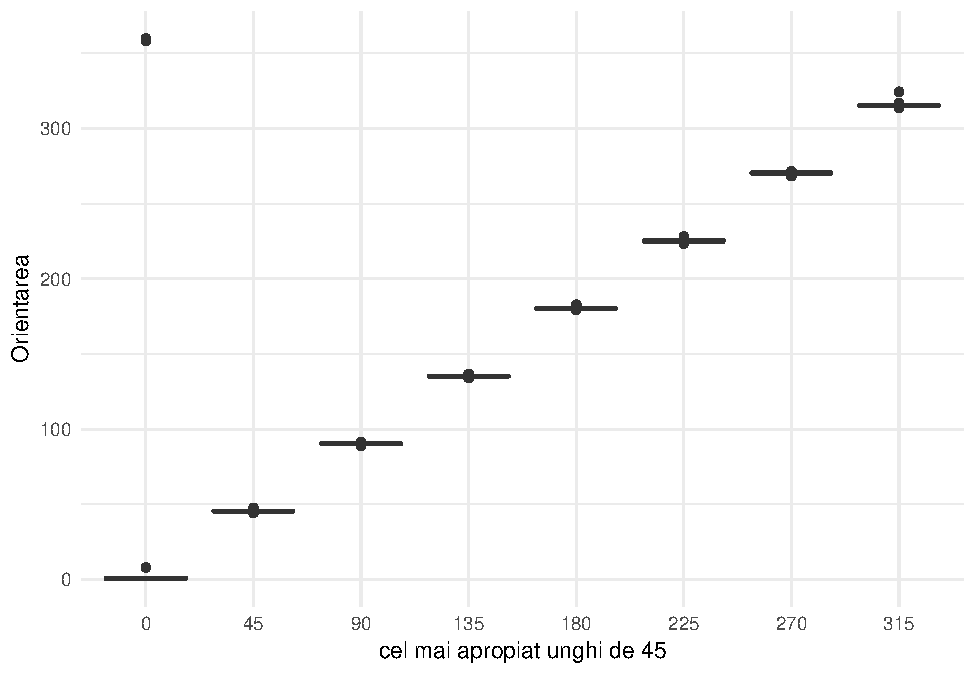
\includegraphics[width=0.9\linewidth]{Lab_5_files/figure-latex/unnamed-chunk-19-1} \end{center}

\subsection{Exemplul 2}\label{exemplul-2}

\begin{center}\rule{0.5\linewidth}{\linethickness}\end{center}

\begin{quote}
În acest exemplu vom folosi setul de date \emph{Cholesterol} din
pachetul \texttt{multcomp} (datele se pot descărca de
\href{data/cholesterol.csv}{aici}). Datele prezintă cu cât s-a redus
nivelul de colesterol (variabila \emph{response}) la 50 de pacienți ce
au urmat 5 tratamente de reducere a colesterolului. Trei dintre
tratamente au implicat același medicament administrat în moduri
diferite: 20 mg o dată pe zi (\emph{1time}), 10 mg de două ori pe zi
(\emph{2time}) sau 5 mg de patru ori pe zi (\emph{4time}). Celelalte
două tratamente au constat din medicamente alternative diferite
(\emph{drugD} și \emph{drugE}). Care tratament a produs cea mai mare
reducere a colesterolului ?
\end{quote}

Începem prin a citi setul de date:

\begin{Shaded}
\begin{Highlighting}[]
\NormalTok{cholesterol =}\StringTok{ }\KeywordTok{read.csv}\NormalTok{(}\StringTok{"data/cholesterol.csv"}\NormalTok{, }\DataTypeTok{stringsAsFactors =} \OtherTok{FALSE}\NormalTok{)}
\KeywordTok{head}\NormalTok{(cholesterol)}
\end{Highlighting}
\end{Shaded}

\begin{verbatim}
##     trt response
## 1 1time   3.8612
## 2 1time  10.3868
## 3 1time   5.9059
## 4 1time   3.0609
## 5 1time   7.7204
## 6 1time   2.7139
\end{verbatim}

Vedem câte observații avem pentru fiecare tratament:

\begin{Shaded}
\begin{Highlighting}[]
\KeywordTok{table}\NormalTok{(cholesterol$trt)}
\end{Highlighting}
\end{Shaded}

\begin{verbatim}
## 
##  1time 2times 4times  drugD  drugE 
##     10     10     10     10     10
\end{verbatim}

Observăm că fiecare tratament a fost administrat la câte 10 pacienți
(suntem în contextul unui \emph{plan de experiență echilibrat}).

Calculăm:

\begin{itemize}
\tightlist
\item
  numărul total de observații (\(n\)) și numărul de observații din
  fiecare grup (\(n_i\))
\end{itemize}

\begin{Shaded}
\begin{Highlighting}[]
\NormalTok{n =}\StringTok{ }\KeywordTok{length}\NormalTok{(cholesterol$trt) }\CommentTok{# nr total de observații}

\CommentTok{# nr de observatii pe grup}
\NormalTok{ng =}\StringTok{ }\KeywordTok{table}\NormalTok{(cholesterol$trt)}
\end{Highlighting}
\end{Shaded}

\begin{itemize}
\tightlist
\item
  media fiecărui grup (\(\bar{y}_i\))
\end{itemize}

\begin{Shaded}
\begin{Highlighting}[]
\CommentTok{# media globala}
\NormalTok{my =}\StringTok{ }\KeywordTok{mean}\NormalTok{(cholesterol$response)}

\CommentTok{# media pe grup }
\NormalTok{myg =}\StringTok{ }\KeywordTok{tapply}\NormalTok{(cholesterol$response, cholesterol$trt, mean)}
\NormalTok{myg}
\end{Highlighting}
\end{Shaded}

\begin{verbatim}
##    1time   2times   4times    drugD    drugE 
##  5.78197  9.22497 12.37478 15.36117 20.94752
\end{verbatim}

Se observă că drugE a produs (în medie) cea mai mare reducere a
colesterolului pe când 1time a produs-o pe cea mai mică.

\begin{itemize}
\tightlist
\item
  abaterea standard a fiecărui grup
\end{itemize}

\begin{Shaded}
\begin{Highlighting}[]
\CommentTok{# sd pe grup }
\NormalTok{syg =}\StringTok{ }\KeywordTok{tapply}\NormalTok{(cholesterol$response, cholesterol$trt, sd)}
\NormalTok{syg}
\end{Highlighting}
\end{Shaded}

\begin{verbatim}
##    1time   2times   4times    drugD    drugE 
## 2.878113 3.483054 2.923119 3.454636 3.345003
\end{verbatim}

Se observă că abaterile standard sunt relativ constante pentru cele 5
tratamente, luând valori între 2.9 și 3.5.

\begin{center}\includegraphics[width=0.9\linewidth]{Lab_5_files/figure-latex/unnamed-chunk-25-1} \end{center}

Avem tabelul \emph{ANOVA}:

\begin{Shaded}
\begin{Highlighting}[]
\NormalTok{anova_model =}\StringTok{ }\KeywordTok{aov}\NormalTok{(response~trt, }\DataTypeTok{data =} \NormalTok{cholesterol)}

\KeywordTok{summary}\NormalTok{(anova_model)}
\end{Highlighting}
\end{Shaded}

\begin{verbatim}
##             Df Sum Sq Mean Sq F value   Pr(>F)    
## trt          4 1351.4   337.8   32.43 9.82e-13 ***
## Residuals   45  468.8    10.4                     
## ---
## Signif. codes:  0 '***' 0.001 '**' 0.01 '*' 0.05 '.' 0.1 ' ' 1
\end{verbatim}

Testul ANOVA (F) pentru tratament (trt) este semnificativ (\(p<0.001\)),
ilustrând că cele 5 tratamente nu sunt la fel de eficiente.

Reducerea medie de colesterol pentru cele 5 tratamente împreună cu
intervalele de încredere de nivel de încredere de \(95\%\)
corespunzătoare:

\begin{center}\includegraphics[width=0.9\linewidth]{Lab_5_files/figure-latex/unnamed-chunk-27-1} \end{center}

\subsubsection*{Verificarea ipotezelor
ANOVA}\label{verificarea-ipotezelor-anova-1}
\addcontentsline{toc}{subsubsection}{Verificarea ipotezelor ANOVA}

În ANOVA cu un factor, se presupune că variabila răspuns este
repartizată normal cu aceeași varianță în fiecare grup. Pentru testarea
normalității putem folosi ca metodă grafică \texttt{Q-Q\ plot}-ul:

\begin{center}\includegraphics[width=0.9\linewidth]{Lab_5_files/figure-latex/unnamed-chunk-28-1} \end{center}

De asemenea ipoteza de normalitate poate fi testată și cu testul
\emph{Shapiro-Wilks} sau \emph{Shapiro-Francia}:

\begin{Shaded}
\begin{Highlighting}[]
\NormalTok{anova_model_chol =}\StringTok{ }\KeywordTok{aov}\NormalTok{(response~trt, }\DataTypeTok{data =} \NormalTok{cholesterol)}
\KeywordTok{shapiro.test}\NormalTok{(}\KeywordTok{residuals}\NormalTok{(anova_model_chol))}
\end{Highlighting}
\end{Shaded}

\begin{verbatim}
## 
##  Shapiro-Wilk normality test
## 
## data:  residuals(anova_model_chol)
## W = 0.98864, p-value = 0.9094
\end{verbatim}

Pentru testarea ipotezei de homoscedasticitate aplicăm \emph{testul lui
Bartlett}(i.e.~verificăm \(H_0: \sigma_1=\cdots=\sigma_r\)):

\begin{Shaded}
\begin{Highlighting}[]
\KeywordTok{bartlett.test}\NormalTok{(response~trt, }\DataTypeTok{data =} \NormalTok{cholesterol)}
\end{Highlighting}
\end{Shaded}

\begin{verbatim}
## 
##  Bartlett test of homogeneity of variances
## 
## data:  response by trt
## Bartlett's K-squared = 0.57975, df = 4, p-value = 0.9653
\end{verbatim}

Testul lui Bartlett ne indică faptul că varianțele în cele 5 grupuri nu
diferă semnificativ (\(p = 0.97\)). Pentru testarea ipotezei de
omogenitate se mai pot folosi și alte teste printre care includem
\emph{testul lui Fligner-Killeen} (\texttt{fligner.test}) și
\emph{testul Brown-Forsythe} (funcția \texttt{hov()} din pachetul
\texttt{HH}). Ambele teste întorc același rezultat:

\begin{Shaded}
\begin{Highlighting}[]
\KeywordTok{fligner.test}\NormalTok{(response~}\KeywordTok{as.factor}\NormalTok{(trt), }\DataTypeTok{data =} \NormalTok{cholesterol)}
\end{Highlighting}
\end{Shaded}

\begin{verbatim}
## 
##  Fligner-Killeen test of homogeneity of variances
## 
## data:  response by as.factor(trt)
## Fligner-Killeen:med chi-squared = 0.74277, df = 4, p-value = 0.946
\end{verbatim}

\begin{Shaded}
\begin{Highlighting}[]
\KeywordTok{hov}\NormalTok{(response~trt, }\DataTypeTok{data =} \NormalTok{cholesterol) }\CommentTok{# hov = homogeneity of variance}
\end{Highlighting}
\end{Shaded}

\begin{verbatim}
## 
##  hov: Brown-Forsyth
## 
## data:  response
## F = 0.075477, df:trt = 4, df:Residuals = 45, p-value = 0.9893
## alternative hypothesis: variances are not identical
\end{verbatim}

\subsubsection*{Comparări multiple}\label{comparari-multiple}
\addcontentsline{toc}{subsubsection}{Comparări multiple}

Testul F din ANOVA pentru tratamente ne spune că cele 5 tipuri de
medicamente nu sunt la fel de eficiente, însă nu ne spune care dintre
ele diferă față de celelalte. Pentru a răspunde la această întrebare vom
folosi metodologia testării multiple. Ca exemplu vom folosi \emph{Testul
lui Tukey HSD} (Honestly Significant Difference), test care permite
compararea tuturor perechilor de diferențe dintre mediile grupurilor:

\begin{Shaded}
\begin{Highlighting}[]
\KeywordTok{TukeyHSD}\NormalTok{(anova_model_chol)}
\end{Highlighting}
\end{Shaded}

\begin{verbatim}
##   Tukey multiple comparisons of means
##     95% family-wise confidence level
## 
## Fit: aov(formula = response ~ trt, data = cholesterol)
## 
## $trt
##                   diff        lwr       upr     p adj
## 2times-1time   3.44300 -0.6582817  7.544282 0.1380949
## 4times-1time   6.59281  2.4915283 10.694092 0.0003542
## drugD-1time    9.57920  5.4779183 13.680482 0.0000003
## drugE-1time   15.16555 11.0642683 19.266832 0.0000000
## 4times-2times  3.14981 -0.9514717  7.251092 0.2050382
## drugD-2times   6.13620  2.0349183 10.237482 0.0009611
## drugE-2times  11.72255  7.6212683 15.823832 0.0000000
## drugD-4times   2.98639 -1.1148917  7.087672 0.2512446
## drugE-4times   8.57274  4.4714583 12.674022 0.0000037
## drugE-drugD    5.58635  1.4850683  9.687632 0.0030633
\end{verbatim}

Observăm că reducerea medie a colesterolului pentru tratamentele
\emph{1time} și \emph{2times} nu este semnificativă (\(p=0.138\)) pe
când reducerea medie a colesterolului pentru tratamentele \emph{1time}
și \emph{4times} este semnificativă (\(p<0.001\)).

Aceste diferențe se pot observa și grafic:

\begin{center}\includegraphics[width=0.9\linewidth]{Lab_5_files/figure-latex/unnamed-chunk-35-1} \end{center}

Trebuie menționat că sunt mai multe metode pentru comparări multiple:
\emph{metoda Bonferroni}, \emph{metoda contrastelor liniare},
\emph{metoda bazată pe statistici de rang}, \emph{metoda Newman Keuls}
etc.

\section{Analiză de varianță cu doi factori (two-way
ANOVA)}\label{analiza-de-varianta-cu-doi-factori-two-way-anova}

\begin{center}\rule{0.5\linewidth}{\linethickness}\end{center}

\begin{center}\rule{0.5\linewidth}{\linethickness}\end{center}

Analiza de varianță cu doi factori poate fi văzută ca o generalizare a
analizei de varianță cu un factor, în acest model subiecții fiind
distribuiți în grupe rezultate din încrucișarea modalităților celor doi
factori.

Ca și în cazul one-way ANOVA, condițiile de aplicare rămân aceleași:
populații normale de aceeași varianță și eșantioane independente.

\subsection{Exemplul 1}\label{exemplul-1-1}

\begin{center}\rule{0.5\linewidth}{\linethickness}\end{center}

\begin{quote}
În acest exemplu vom folosi setul de date
\href{http://jn.nutrition.org/content/33/5/491.full.pdf}{\texttt{ToothGrowth}}
din pachetul de bază. Datele fac referire la 60 de porcușori de guinea
care sunt repartizați aleator să primească unul din cele trei nivele de
Vitamina C (0.5, 1 și 2 mg) prin una din cele două modalități propuse
(suc de portocale - OJ sau o soluție apoasă de acid ascorbic - VC), cu
restricția ca fiecare combinație de tratament să fie atribuită la 10
porcușori. Vrem să investigăm efectul Vitaminei C asupra creșterii
dinților porcușorilor de guinea prin cele două metode de livrare.
\end{quote}

Atașăm setul de date \texttt{ToothGrowth}:

\begin{Shaded}
\begin{Highlighting}[]
\KeywordTok{data}\NormalTok{(}\StringTok{"ToothGrowth"}\NormalTok{)}
\KeywordTok{attach}\NormalTok{(ToothGrowth)}

\KeywordTok{head}\NormalTok{(ToothGrowth)}
\end{Highlighting}
\end{Shaded}

\begin{verbatim}
##    len supp dose
## 1  4.2   VC  0.5
## 2 11.5   VC  0.5
## 3  7.3   VC  0.5
## 4  5.8   VC  0.5
## 5  6.4   VC  0.5
## 6 10.0   VC  0.5
\end{verbatim}

Structura setului de date este:

\begin{Shaded}
\begin{Highlighting}[]
\KeywordTok{str}\NormalTok{(ToothGrowth)}
\end{Highlighting}
\end{Shaded}

\begin{verbatim}
## 'data.frame':    60 obs. of  3 variables:
##  $ len : num  4.2 11.5 7.3 5.8 6.4 10 11.2 11.2 5.2 7 ...
##  $ supp: Factor w/ 2 levels "OJ","VC": 2 2 2 2 2 2 2 2 2 2 ...
##  $ dose: num  0.5 0.5 0.5 0.5 0.5 0.5 0.5 0.5 0.5 0.5 ...
\end{verbatim}

unde \texttt{len} este variabila dependentă (variabila răspuns) iar
\texttt{supp} și \texttt{dose} sunt variabilele explicative (cei doi
factori).

Descompunerea erorii în modelul ANOVA cu doi factori este:

\[
\begin{aligned}
  \underbrace{\sum_{i=1}^{r}\sum_{j=1}^{c}\sum_{k=1}^{s}(Y_{ijk}-\bar{Y}_{\cdot\cdot\cdot})^2}_{SS_T} &= \underbrace{sc\sum_{i=1}^{r}(\bar{Y}_{i\cdot\cdot}-\bar{Y}_{\cdot\cdot\cdot})^2}_{SS_A}+\underbrace{sr\sum_{j=1}^{c}(\bar{Y}_{\cdot j\cdot}-\bar{Y}_{\cdot\cdot\cdot})^2}_{SS_B}\\
  &\;\;\;\;\; + \underbrace{s\sum_{i=1}^{r}\sum_{j=1}^{c}(\bar{Y}_{i j\cdot}-\bar{Y}_{i\cdot\cdot}-\bar{Y}_{\cdot j\cdot}+\bar{Y}_{\cdot\cdot\cdot})^2}_{SS_{A\times B}} + \underbrace{\sum_{i=1}^{r}\sum_{j=1}^{c}\sum_{k=1}^{s}(Y_{ijk}-\bar{Y}_{i j\cdot})^2}_{SS_W}
\end{aligned}
\]

Tabelul ANOVA devine:

\begin{longtable}[]{@{}ccccc@{}}
\toprule
Sursa & DF & SS & MS & F\_test\tabularnewline
\midrule
\endhead
\(A\) & \(r-1\) & \(SS_A\) & \(MS_A\) &
\(\frac{MS_A}{MS_W}\)\tabularnewline
\(B\) & \(c-1\) & \(SS_B\) & \(MS_B\) &
\(\frac{MS_B}{MS_W}\)\tabularnewline
\(A\times B\) & \((r-1)(c-1)\) & \(SS_{A\times B}\) & \(MS_{A\times B}\)
& \(\frac{MS_{A\times B}}{MS_W}\)\tabularnewline
\(W\) & \(rc(s-1)\) & \(SS_W\) & \(MS_W\) &\tabularnewline
\(Total\) & \(rcs-1\) & \(SS_T\) & &\tabularnewline
\bottomrule
\end{longtable}

Pentru a calcula numărul de observații din fiecare încrucișare de
categorii vom folosi funcția \texttt{table}:

\begin{Shaded}
\begin{Highlighting}[]
\CommentTok{# nr de categorii pentru fiecare factor}
\NormalTok{r =}\StringTok{ }\DecValTok{2}
\NormalTok{c =}\StringTok{ }\DecValTok{3}
\NormalTok{s =}\StringTok{ }\DecValTok{10}

\CommentTok{# nr de observatii pentru factorul A}
\NormalTok{n_i =}\StringTok{ }\KeywordTok{table}\NormalTok{(supp)}
\NormalTok{n_i}
\end{Highlighting}
\end{Shaded}

\begin{verbatim}
## supp
## OJ VC 
## 30 30
\end{verbatim}

\begin{Shaded}
\begin{Highlighting}[]
\CommentTok{# nr de observatii pentru factorul B}
\NormalTok{n_j =}\StringTok{ }\KeywordTok{table}\NormalTok{(dose)}
\NormalTok{n_j}
\end{Highlighting}
\end{Shaded}

\begin{verbatim}
## dose
## 0.5   1   2 
##  20  20  20
\end{verbatim}

\begin{Shaded}
\begin{Highlighting}[]
\CommentTok{# nr de observatii pentru fiecare incrucisare a factorilor A si B}
\NormalTok{n_ij =}\StringTok{ }\KeywordTok{table}\NormalTok{(supp, dose)}
\NormalTok{n_ij}
\end{Highlighting}
\end{Shaded}

\begin{verbatim}
##     dose
## supp 0.5  1  2
##   OJ  10 10 10
##   VC  10 10 10
\end{verbatim}

de unde observăm că suntem în contextul unui plan de experiență
echilibrat (\(r = 2\), \(c = 3\) și \(s = 10\)).

Vom calcula mediile \(\bar{Y}_{i j\cdot}\), \(\bar{Y}_{i \cdot\cdot}\),
\(\bar{Y}_{\cdot j\cdot}\) și \(\bar{Y}_{\cdot\cdot\cdot}\):

\begin{itemize}
\tightlist
\item
  pentru \(\bar{Y}_{\cdot\cdot\cdot}\)
\end{itemize}

\begin{Shaded}
\begin{Highlighting}[]
\NormalTok{m_T =}\StringTok{ }\KeywordTok{mean}\NormalTok{(len)}
\NormalTok{m_T}
\end{Highlighting}
\end{Shaded}

\begin{verbatim}
## [1] 18.81333
\end{verbatim}

\begin{itemize}
\tightlist
\item
  pentru \(\bar{Y}_{i \cdot\cdot}\)
\end{itemize}

\begin{Shaded}
\begin{Highlighting}[]
\NormalTok{m_i =}\StringTok{ }\KeywordTok{tapply}\NormalTok{(len, supp, mean)}
\NormalTok{m_i}
\end{Highlighting}
\end{Shaded}

\begin{verbatim}
##       OJ       VC 
## 20.66333 16.96333
\end{verbatim}

\begin{itemize}
\tightlist
\item
  pentru \(\bar{Y}_{\cdot j\cdot}\)
\end{itemize}

\begin{Shaded}
\begin{Highlighting}[]
\NormalTok{m_j =}\StringTok{ }\KeywordTok{tapply}\NormalTok{(len, dose, mean)}
\NormalTok{m_j}
\end{Highlighting}
\end{Shaded}

\begin{verbatim}
##    0.5      1      2 
## 10.605 19.735 26.100
\end{verbatim}

\begin{itemize}
\tightlist
\item
  pentru \(\bar{Y}_{i j\cdot}\)
\end{itemize}

\begin{Shaded}
\begin{Highlighting}[]
\NormalTok{m_ij =}\StringTok{ }\KeywordTok{tapply}\NormalTok{(len, }\KeywordTok{list}\NormalTok{(supp, dose), mean)}
\NormalTok{m_ij}
\end{Highlighting}
\end{Shaded}

\begin{verbatim}
##      0.5     1     2
## OJ 13.23 22.70 26.06
## VC  7.98 16.77 26.14
\end{verbatim}

\begin{center}\includegraphics[width=0.9\linewidth]{Lab_5_files/figure-latex/unnamed-chunk-46-1} \end{center}

Calculăm \(SS_W\), \(df_W\) și \(MS_W\):

\begin{Shaded}
\begin{Highlighting}[]
\NormalTok{y =}\StringTok{ }\NormalTok{len}

\NormalTok{rep_ij =}\StringTok{ }\KeywordTok{c}\NormalTok{(}\KeywordTok{rep}\NormalTok{(m_ij[}\StringTok{"VC"}\NormalTok{,], n_ij[}\StringTok{"VC"}\NormalTok{,]), }\KeywordTok{rep}\NormalTok{(m_ij[}\StringTok{"OJ"}\NormalTok{,], n_ij[}\StringTok{"OJ"}\NormalTok{,]))}

\NormalTok{SS_W =}\StringTok{ }\KeywordTok{sum}\NormalTok{((y-rep_ij)^}\DecValTok{2}\NormalTok{)}
\KeywordTok{cat}\NormalTok{(}\StringTok{"SS_W = "}\NormalTok{, SS_W,}\StringTok{"}\CharTok{\textbackslash{}n}\StringTok{"}\NormalTok{)}
\end{Highlighting}
\end{Shaded}

\begin{verbatim}
## SS_W =  712.106
\end{verbatim}

\begin{Shaded}
\begin{Highlighting}[]
\NormalTok{df_W =}\StringTok{ }\NormalTok{r*c*(s}\DecValTok{-1}\NormalTok{)}
\KeywordTok{cat}\NormalTok{(}\StringTok{"df_W = "}\NormalTok{, df_W,}\StringTok{"}\CharTok{\textbackslash{}n}\StringTok{"}\NormalTok{)}
\end{Highlighting}
\end{Shaded}

\begin{verbatim}
## df_W =  54
\end{verbatim}

\begin{Shaded}
\begin{Highlighting}[]
\NormalTok{MS_W =}\StringTok{ }\NormalTok{SS_W/df_W}
\KeywordTok{cat}\NormalTok{(}\StringTok{"MS_W = "}\NormalTok{, MS_W,}\StringTok{"}\CharTok{\textbackslash{}n}\StringTok{"}\NormalTok{)}
\end{Highlighting}
\end{Shaded}

\begin{verbatim}
## MS_W =  13.18715
\end{verbatim}

Calculăm \(SS_A\), \(df_A\) și \(MS_A\):

\begin{Shaded}
\begin{Highlighting}[]
\NormalTok{SS_A =}\StringTok{ }\NormalTok{s*c*}\KeywordTok{sum}\NormalTok{((m_i-m_T)^}\DecValTok{2}\NormalTok{)}
\KeywordTok{cat}\NormalTok{(}\StringTok{"SS_A = "}\NormalTok{, SS_A,}\StringTok{"}\CharTok{\textbackslash{}n}\StringTok{"}\NormalTok{)}
\end{Highlighting}
\end{Shaded}

\begin{verbatim}
## SS_A =  205.35
\end{verbatim}

\begin{Shaded}
\begin{Highlighting}[]
\NormalTok{df_A =}\StringTok{ }\NormalTok{r}\DecValTok{-1}
\KeywordTok{cat}\NormalTok{(}\StringTok{"df_A = "}\NormalTok{, df_A,}\StringTok{"}\CharTok{\textbackslash{}n}\StringTok{"}\NormalTok{)}
\end{Highlighting}
\end{Shaded}

\begin{verbatim}
## df_A =  1
\end{verbatim}

\begin{Shaded}
\begin{Highlighting}[]
\NormalTok{MS_A =}\StringTok{ }\NormalTok{SS_A/df_A}
\KeywordTok{cat}\NormalTok{(}\StringTok{"MS_A = "}\NormalTok{, MS_A,}\StringTok{"}\CharTok{\textbackslash{}n}\StringTok{"}\NormalTok{)}
\end{Highlighting}
\end{Shaded}

\begin{verbatim}
## MS_A =  205.35
\end{verbatim}

Calculăm \(SS_B\), \(df_B\) și \(MS_B\):

\begin{Shaded}
\begin{Highlighting}[]
\NormalTok{SS_B =}\StringTok{ }\NormalTok{s*r*}\KeywordTok{sum}\NormalTok{((m_j-m_T)^}\DecValTok{2}\NormalTok{)}
\KeywordTok{cat}\NormalTok{(}\StringTok{"SS_B = "}\NormalTok{, SS_B,}\StringTok{"}\CharTok{\textbackslash{}n}\StringTok{"}\NormalTok{)}
\end{Highlighting}
\end{Shaded}

\begin{verbatim}
## SS_B =  2426.434
\end{verbatim}

\begin{Shaded}
\begin{Highlighting}[]
\NormalTok{df_B =}\StringTok{ }\NormalTok{c}\DecValTok{-1}
\KeywordTok{cat}\NormalTok{(}\StringTok{"df_B = "}\NormalTok{, df_B,}\StringTok{"}\CharTok{\textbackslash{}n}\StringTok{"}\NormalTok{)}
\end{Highlighting}
\end{Shaded}

\begin{verbatim}
## df_B =  2
\end{verbatim}

\begin{Shaded}
\begin{Highlighting}[]
\NormalTok{MS_B =}\StringTok{ }\NormalTok{SS_B/df_B}
\KeywordTok{cat}\NormalTok{(}\StringTok{"MS_B = "}\NormalTok{, SS_B,}\StringTok{"}\CharTok{\textbackslash{}n}\StringTok{"}\NormalTok{)}
\end{Highlighting}
\end{Shaded}

\begin{verbatim}
## MS_B =  2426.434
\end{verbatim}

Calculăm \(SS_{A\times B}\), \(df_{A\times B}\) și \(MS_{A\times B}\):

\begin{Shaded}
\begin{Highlighting}[]
\NormalTok{v =}\StringTok{ }\NormalTok{m_ij -}\StringTok{ }\KeywordTok{matrix}\NormalTok{(}\KeywordTok{rep}\NormalTok{(m_i, c), }\DataTypeTok{ncol =} \NormalTok{c) -}\StringTok{ }
\StringTok{  }\KeywordTok{matrix}\NormalTok{(}\KeywordTok{rep}\NormalTok{(m_j, r), }\DataTypeTok{nrow =} \NormalTok{r, }\DataTypeTok{byrow =} \NormalTok{T) +}\StringTok{ }\NormalTok{m_T}
\NormalTok{SS_AB =}\StringTok{ }\NormalTok{s*}\KeywordTok{sum}\NormalTok{(v^}\DecValTok{2}\NormalTok{)}
\KeywordTok{cat}\NormalTok{(}\StringTok{"SS_AB = "}\NormalTok{, SS_AB,}\StringTok{"}\CharTok{\textbackslash{}n}\StringTok{"}\NormalTok{)}
\end{Highlighting}
\end{Shaded}

\begin{verbatim}
## SS_AB =  108.319
\end{verbatim}

\begin{Shaded}
\begin{Highlighting}[]
\NormalTok{df_AB =}\StringTok{ }\NormalTok{(r}\DecValTok{-1}\NormalTok{)*(c}\DecValTok{-1}\NormalTok{)}
\KeywordTok{cat}\NormalTok{(}\StringTok{"df_AB = "}\NormalTok{, df_AB,}\StringTok{"}\CharTok{\textbackslash{}n}\StringTok{"}\NormalTok{)}
\end{Highlighting}
\end{Shaded}

\begin{verbatim}
## df_AB =  2
\end{verbatim}

\begin{Shaded}
\begin{Highlighting}[]
\NormalTok{MS_AB =}\StringTok{ }\NormalTok{SS_AB/df_AB}
\KeywordTok{cat}\NormalTok{(}\StringTok{"MS_AB = "}\NormalTok{, SS_AB,}\StringTok{"}\CharTok{\textbackslash{}n}\StringTok{"}\NormalTok{)}
\end{Highlighting}
\end{Shaded}

\begin{verbatim}
## MS_AB =  108.319
\end{verbatim}

Calculăm \(SS_T\):

\begin{Shaded}
\begin{Highlighting}[]
\NormalTok{SS_T =}\StringTok{ }\NormalTok{SS_A +}\StringTok{ }\NormalTok{SS_B +}\StringTok{ }\NormalTok{SS_AB +}\StringTok{ }\NormalTok{SS_W}
\KeywordTok{cat}\NormalTok{(}\StringTok{"SS_T = "}\NormalTok{, SS_T,}\StringTok{"}\CharTok{\textbackslash{}n}\StringTok{"}\NormalTok{)}
\end{Highlighting}
\end{Shaded}

\begin{verbatim}
## SS_T =  3452.209
\end{verbatim}

\begin{Shaded}
\begin{Highlighting}[]
\CommentTok{# verificam prin formula}
\KeywordTok{sum}\NormalTok{((y-m_T)^}\DecValTok{2}\NormalTok{)}
\end{Highlighting}
\end{Shaded}

\begin{verbatim}
## [1] 3452.209
\end{verbatim}

Calculăm tabelul ANOVA cu funcția \texttt{aov}:

\begin{Shaded}
\begin{Highlighting}[]
\NormalTok{ToothGrowth$dose =}\StringTok{ }\KeywordTok{as.factor}\NormalTok{(ToothGrowth$dose)}
\NormalTok{ToothGrowth$supp =}\StringTok{ }\KeywordTok{as.factor}\NormalTok{(ToothGrowth$supp)}

\NormalTok{model_anova_2w =}\StringTok{ }\KeywordTok{aov}\NormalTok{(len~supp*dose, }\DataTypeTok{data =} \NormalTok{ToothGrowth)}

\KeywordTok{summary}\NormalTok{(model_anova_2w)}
\end{Highlighting}
\end{Shaded}

\begin{verbatim}
##             Df Sum Sq Mean Sq F value   Pr(>F)    
## supp         1  205.4   205.4  15.572 0.000231 ***
## dose         2 2426.4  1213.2  92.000  < 2e-16 ***
## supp:dose    2  108.3    54.2   4.107 0.021860 *  
## Residuals   54  712.1    13.2                     
## ---
## Signif. codes:  0 '***' 0.001 '**' 0.01 '*' 0.05 '.' 0.1 ' ' 1
\end{verbatim}

Tabelul ANOVA de mai sus ne arată că atât efectele principale
(\texttt{supp} și \texttt{dose}) cât și interacția dintre cei doi
factori (\texttt{supp:dose}) sunt semnificative.

Pentru a vedea interacția dintre cei doi factori putem să folosim
funcția \texttt{interaction.plot}:

\begin{Shaded}
\begin{Highlighting}[]
\KeywordTok{interaction.plot}\NormalTok{(dose, supp, len, }\DataTypeTok{type=}\StringTok{"b"}\NormalTok{,}
        \DataTypeTok{col=}\KeywordTok{c}\NormalTok{(}\StringTok{"brown3"}\NormalTok{,}\StringTok{"darkgray"}\NormalTok{), }\DataTypeTok{pch=}\KeywordTok{c}\NormalTok{(}\DecValTok{16}\NormalTok{, }\DecValTok{18}\NormalTok{),}
        \DataTypeTok{main =} \StringTok{"Interactia dintre doza de Vitamina C si tipul de suplement"}\NormalTok{,}
        \DataTypeTok{xlab =} \StringTok{"Doza de Vitamina C in mg"}\NormalTok{,}
        \DataTypeTok{ylab =} \StringTok{"Media lungimii dintilor"}\NormalTok{)}
\end{Highlighting}
\end{Shaded}

\begin{center}\includegraphics[width=0.9\linewidth]{Lab_5_files/figure-latex/unnamed-chunk-53-1} \end{center}

Dacă vrem să includem și intervalele de încredere atunci avem:

\begin{center}\includegraphics[width=0.9\linewidth]{Lab_5_files/figure-latex/unnamed-chunk-54-1} \end{center}

Graficele ne arată că dinții de la porcușorii de guinea cresc cu doza de
Vitamina C atât pentru sucul de portocale cât și pentru soluția de acid
ascorbic. Pentru dozele de 0.5 și 1 mg, sucul de portocale produce în
medie o creștere mai mare a dinților decât soluția de acid ascorbic.
Pentru doza de 2 mg, ambele metode produc aceeași creștere.

\subsubsection{Verificarea ipotezelor
ANOVA}\label{verificarea-ipotezelor-anova-2}

\begin{center}\rule{0.5\linewidth}{\linethickness}\end{center}

Vom începe prin a testa \textbf{condiția de normalitate} a
observațiilor. Pentru aceasta vom folosi testul \texttt{Shapiro-Wilks}
(funcția \texttt{shapiro.test}) și metoda grafică a \emph{dreptei lui
Henry} (Q-Q plot). Ca și în cazul ANOVA cu un factor, vom testa
normalitatea datelor pentru toate datele și nu pentru fiecare eșantion
în parte. În acest sens va trebui să calculăm reziduurile:

\[
  \hat{e}_{ijk} = y_{ijk}-\bar{y}_{ij\cdot}
\]

lucru care poate fi realizat sau prin calcul direct:

\begin{Shaded}
\begin{Highlighting}[]
\NormalTok{res_model_direct =}\StringTok{ }\NormalTok{y-rep_ij}
\end{Highlighting}
\end{Shaded}

sau folosind funcția residuals:

\begin{Shaded}
\begin{Highlighting}[]
\NormalTok{res_model =}\StringTok{ }\KeywordTok{residuals}\NormalTok{(model_anova_2w)}
\end{Highlighting}
\end{Shaded}

Aplicăm testul Shapiro-Wilks pentru reziduuri și obținem:

\begin{Shaded}
\begin{Highlighting}[]
\KeywordTok{shapiro.test}\NormalTok{(res_model)}
\end{Highlighting}
\end{Shaded}

\begin{verbatim}
## 
##  Shapiro-Wilk normality test
## 
## data:  res_model
## W = 0.98499, p-value = 0.6694
\end{verbatim}

de unde concluzionăm că ipoteza de normalitate este satisfăcută. Aceeași
concluzie o obținem și prin metoda grafică:

\begin{Shaded}
\begin{Highlighting}[]
\KeywordTok{qqPlot}\NormalTok{(}\KeywordTok{lm}\NormalTok{(len~supp*dose, }\DataTypeTok{data =} \NormalTok{ToothGrowth), }
       \DataTypeTok{simulate =} \OtherTok{TRUE}\NormalTok{,}
       \DataTypeTok{main =} \StringTok{"Q-Q plot"}\NormalTok{,}
       \DataTypeTok{xlab =} \StringTok{"Cuantile teoretice"}\NormalTok{, }
       \DataTypeTok{ylab =} \StringTok{"Reziduurile standardizate"}\NormalTok{)}
\end{Highlighting}
\end{Shaded}

\includegraphics{Lab_5_files/figure-latex/unnamed-chunk-58-1.pdf}

Trebuie menționat că în cazul în care ipoteza de normalitate era
respinsă atunci puteam folosi testul neparametric
\texttt{Kruskal-Wallis} (funcția \texttt{kruskal.test}) ca alternativă
la ANOVA.

Pentru a verifica \textbf{condiția de omogenitate} a datelor
(homoscedasticitatea) pentru fiecare factor în parte folosim unul din
testele următoare: \emph{testul lui Bartlett} (funcția
\texttt{bartlett.test}), \emph{testul lui Fligner-Killeen} (funcția
\texttt{fligner.test}), \emph{testul lui Levene} (funcția
\texttt{leveneTest} din pachetul \texttt{car}) sau \emph{testul
Brown-Forsythe} (funcția \texttt{leveneTest} din pachetul \texttt{car}
sau funcția \texttt{hov()} din pachetul \texttt{HH}). Obținem:

\begin{itemize}
\tightlist
\item
  testul lui Bartlett
\end{itemize}

\begin{Shaded}
\begin{Highlighting}[]
\KeywordTok{bartlett.test}\NormalTok{(len~supp, }\DataTypeTok{data =} \NormalTok{ToothGrowth)}
\end{Highlighting}
\end{Shaded}

\begin{verbatim}
## 
##  Bartlett test of homogeneity of variances
## 
## data:  len by supp
## Bartlett's K-squared = 1.4217, df = 1, p-value = 0.2331
\end{verbatim}

\begin{Shaded}
\begin{Highlighting}[]
\KeywordTok{bartlett.test}\NormalTok{(len~dose, }\DataTypeTok{data =} \NormalTok{ToothGrowth)}
\end{Highlighting}
\end{Shaded}

\begin{verbatim}
## 
##  Bartlett test of homogeneity of variances
## 
## data:  len by dose
## Bartlett's K-squared = 0.66547, df = 2, p-value = 0.717
\end{verbatim}

\begin{itemize}
\tightlist
\item
  testul lui Fligner
\end{itemize}

\begin{Shaded}
\begin{Highlighting}[]
\KeywordTok{fligner.test}\NormalTok{(len~supp, }\DataTypeTok{data =} \NormalTok{ToothGrowth)}
\end{Highlighting}
\end{Shaded}

\begin{verbatim}
## 
##  Fligner-Killeen test of homogeneity of variances
## 
## data:  len by supp
## Fligner-Killeen:med chi-squared = 0.97034, df = 1, p-value =
## 0.3246
\end{verbatim}

\begin{Shaded}
\begin{Highlighting}[]
\KeywordTok{fligner.test}\NormalTok{(len~dose, }\DataTypeTok{data =} \NormalTok{ToothGrowth)}
\end{Highlighting}
\end{Shaded}

\begin{verbatim}
## 
##  Fligner-Killeen test of homogeneity of variances
## 
## data:  len by dose
## Fligner-Killeen:med chi-squared = 1.3879, df = 2, p-value = 0.4996
\end{verbatim}

\begin{itemize}
\tightlist
\item
  testul lui Levene (clasic)
\end{itemize}

\begin{Shaded}
\begin{Highlighting}[]
\KeywordTok{leveneTest}\NormalTok{(len~supp, }\DataTypeTok{data =} \NormalTok{ToothGrowth, }\DataTypeTok{center =} \NormalTok{mean)}
\end{Highlighting}
\end{Shaded}

\begin{verbatim}
## Levene's Test for Homogeneity of Variance (center = mean)
##       Df F value Pr(>F)
## group  1  1.0973 0.2992
##       58
\end{verbatim}

\begin{Shaded}
\begin{Highlighting}[]
\KeywordTok{leveneTest}\NormalTok{(len~dose, }\DataTypeTok{data =} \NormalTok{ToothGrowth, }\DataTypeTok{center =} \NormalTok{mean)}
\end{Highlighting}
\end{Shaded}

\begin{verbatim}
## Levene's Test for Homogeneity of Variance (center = mean)
##       Df F value Pr(>F)
## group  2  0.7328  0.485
##       57
\end{verbatim}

\begin{itemize}
\tightlist
\item
  testul lui Brown-Forsythe (similar cu testul lui Levene numai că
  folosește mediana în loc de medie și este mai robust)
\end{itemize}

\begin{Shaded}
\begin{Highlighting}[]
\KeywordTok{leveneTest}\NormalTok{(len~supp, }\DataTypeTok{data =} \NormalTok{ToothGrowth)}
\end{Highlighting}
\end{Shaded}

\begin{verbatim}
## Levene's Test for Homogeneity of Variance (center = median)
##       Df F value Pr(>F)
## group  1  1.2136 0.2752
##       58
\end{verbatim}

\begin{Shaded}
\begin{Highlighting}[]
\KeywordTok{leveneTest}\NormalTok{(len~dose, }\DataTypeTok{data =} \NormalTok{ToothGrowth)}
\end{Highlighting}
\end{Shaded}

\begin{verbatim}
## Levene's Test for Homogeneity of Variance (center = median)
##       Df F value Pr(>F)
## group  2  0.6457 0.5281
##       57
\end{verbatim}

\subsubsection{Comparări multiple}\label{comparari-multiple-1}

\begin{center}\rule{0.5\linewidth}{\linethickness}\end{center}

Am văzut din tabelul ANOVA cu doi factori că atât efectele principale
(\texttt{supp} și \texttt{dose}) cât și interacția dintre cei doi
factori (\texttt{supp:dose}) sunt semnificative. Pentru a vedea care
interacțiune este semnificativă vom folosi metodologia testării
multiple. Vom folosi \emph{Testul lui Tukey HSD} (Honestly Significant
Difference) deoarece suntem în situația unui plan de experiență
echilibrat (în caz contrar am putea folosi \emph{testul lui Scheffe}),
test care permite compararea tuturor perechilor de diferențe dintre
mediile grupurilor:

\begin{Shaded}
\begin{Highlighting}[]
\KeywordTok{TukeyHSD}\NormalTok{(model_anova_2w)}
\end{Highlighting}
\end{Shaded}

\begin{verbatim}
##   Tukey multiple comparisons of means
##     95% family-wise confidence level
## 
## Fit: aov(formula = len ~ supp * dose, data = ToothGrowth)
## 
## $supp
##       diff       lwr       upr     p adj
## VC-OJ -3.7 -5.579828 -1.820172 0.0002312
## 
## $dose
##         diff       lwr       upr   p adj
## 1-0.5  9.130  6.362488 11.897512 0.0e+00
## 2-0.5 15.495 12.727488 18.262512 0.0e+00
## 2-1    6.365  3.597488  9.132512 2.7e-06
## 
## $`supp:dose`
##                diff        lwr        upr     p adj
## VC:0.5-OJ:0.5 -5.25 -10.048124 -0.4518762 0.0242521
## OJ:1-OJ:0.5    9.47   4.671876 14.2681238 0.0000046
## VC:1-OJ:0.5    3.54  -1.258124  8.3381238 0.2640208
## OJ:2-OJ:0.5   12.83   8.031876 17.6281238 0.0000000
## VC:2-OJ:0.5   12.91   8.111876 17.7081238 0.0000000
## OJ:1-VC:0.5   14.72   9.921876 19.5181238 0.0000000
## VC:1-VC:0.5    8.79   3.991876 13.5881238 0.0000210
## OJ:2-VC:0.5   18.08  13.281876 22.8781238 0.0000000
## VC:2-VC:0.5   18.16  13.361876 22.9581238 0.0000000
## VC:1-OJ:1     -5.93 -10.728124 -1.1318762 0.0073930
## OJ:2-OJ:1      3.36  -1.438124  8.1581238 0.3187361
## VC:2-OJ:1      3.44  -1.358124  8.2381238 0.2936430
## OJ:2-VC:1      9.29   4.491876 14.0881238 0.0000069
## VC:2-VC:1      9.37   4.571876 14.1681238 0.0000058
## VC:2-OJ:2      0.08  -4.718124  4.8781238 1.0000000
\end{verbatim}

Observăm, de exemplu, că diferența dintre mediile lungimii dinților
pentru porcușorii de gunineea care au primit o doză de 1 mg de Vitamina
C prin suplementul de suc de portocale și prin suplementul de soluție de
acid ascorbic este semnificativă (VC:1-OJ:1 \(p=0.0073\)) pe când
diferența dintre mediile lungimii dinților pentru porcușorii de gunineea
care au primit o doză de 2 mg și una de 1 mg de Vitamina C prin
suplementul de suc de portocale nu este semnificativă (OJ:2-OJ:1
\(p = 0.318\)).

Aceste diferențe se pot observa și grafic:

\begin{center}\includegraphics[width=0.9\linewidth]{Lab_5_files/figure-latex/unnamed-chunk-64-1} \end{center}

\begin{center}\includegraphics[width=0.9\linewidth]{Lab_5_files/figure-latex/unnamed-chunk-64-2} \end{center}

\begin{center}\includegraphics[width=0.9\linewidth]{Lab_5_files/figure-latex/unnamed-chunk-64-3} \end{center}


\end{document}
